%%%%%%%%%%%%%%%%%%%%%%%%%%%%%%%%%%%%%%%%%
% Journal Article
% LaTeX Template
% Version 1.3 (9/9/13)
%
% This template has been downloaded from:
% http://www.LaTeXTemplates.com
%
% Original author:
% Frits Wenneker (http://www.howtotex.com)
%
% License:
% CC BY-NC-SA 3.0 (http://creativecommons.org/licenses/by-nc-sa/3.0/)
%
%%%%%%%%%%%%%%%%%%%%%%%%%%%%%%%%%%%%%%%%%

%----------------------------------------------------------------------------------------
%	PACKAGES AND OTHER DOCUMENT CONFIGURATIONS
%----------------------------------------------------------------------------------------

\documentclass{article}

\usepackage{mathtools} %tools for mathematical writing
\usepackage{caption}
\usepackage{subfig}
\usepackage{float}
\usepackage{color}
\usepackage{adjustbox}
\usepackage{comment}

\usepackage[sc]{mathpazo} % Use the Palatino font
\usepackage[T1]{fontenc} % Use 8-bit encoding that has 256 glyphs
\linespread{1.05} % Line spacing - Palatino needs more space between lines
\usepackage{microtype} % Slightly tweak font spacing for aesthetics

\usepackage[hmarginratio=1:1,top=32mm,columnsep=20pt]{geometry} % Document margins
%\usepackage{multicol} % Used for the two-column layout of the document
%\usepackage[hang, small,labelfont=bf,up,textfont=it,up]{caption} % Custom captions under/above floats in tables or figures
\usepackage{booktabs} % Horizontal rules in tables
%\usepackage{float} % Required for tables and figures in the multi-column environment - they need to be placed in specific locations with the [H] (e.g. \begin{table}[H])
\usepackage{hyperref} % For hyperlinks in the PDF

\hypersetup{
    colorlinks=true,
    linkcolor=black,
    filecolor=magenta,      
    urlcolor=black,
    citecolor=black
}

\usepackage{lettrine} % The lettrine is the first enlarged letter at the beginning of the text
\usepackage{paralist} % Used for the compactitem environment which makes bullet points with less space between them

\usepackage{abstract} % Allows abstract customization
\renewcommand{\abstractnamefont}{\normalfont\bfseries} % Set the "Abstract" text to bold
\renewcommand{\abstracttextfont}{\normalfont\small\itshape} % Set the abstract itself to small italic text

\usepackage{titlesec} % Allows customization of titles
%\renewcommand\thesection{\Roman{section}} % Roman numerals for the sections
%\renewcommand\thesubsection{\Roman{subsection}} % Roman numerals for subsections
\titleformat{\section}[block]{\large\scshape\centering}{\thesection.}{1em}{} % Change the look of the section titles
\titleformat{\subsection}[block]{\large}{\thesubsection.}{1em}{} % Change the look of the section titles

\usepackage{fancyhdr} % Headers and footers
\pagestyle{fancy} % All pages have headers and footers
\fancyhead{} % Blank out the default header
\fancyfoot{} % Blank out the default footer
\fancyhead[C]{Running title $\bullet$ April 2018 $\bullet$ Vol. XXI, No. 1} % Custom header text
\fancyfoot[RO,LE]{\thepage} % Custom footer text

\usepackage{algorithm}% http://ctan.org/pkg/algorithms
\usepackage{algpseudocode}% http://ctan.org/pkg/algorithmicx

\usepackage[acronym]{glossaries} %Used for the acronyms

\usepackage[titletoc]{appendix}

\DeclarePairedDelimiter\ceil{\lceil}{\rceil}
\DeclarePairedDelimiter\floor{\lfloor}{\rfloor}

%My definitions
%\renewcommand{\tablename}{Table}

\newtheorem{theorem}{Theorem}
\newtheorem{proposition}{Proposition}[section]
\newtheorem{corollary}{Corollary}[theorem]
\newtheorem{remark}{Remark}
\newenvironment{proof}{\begin{trivlist} \item[]\textbf{Proof}
\hspace{0cm} }{\hfill $\Box$ \end{trivlist}}
\newtheorem{mydef}{Definition}[section]
%\newcommand{\eqref}[1]{\mbox{(\ref{#1})}}
\newcommand{\Tr}{\mbox{Tr}}

%Set space between paragraphs
\setlength{\parskip}{2ex}

\usepackage{authblk}

\providecommand{\keywords}[1]{\textbf{\textit{Index terms---}} #1}
%----------------------------------------------------------------------------------------
%	TITLE SECTION
%----------------------------------------------------------------------------------------

\title{A Neural Network-Evolutionary Computation Framework for Remaining Useful Life Estimation}
\author[1]{David Laredo}
\author[1]{Zhaoyin Chen}
\author[2]{Oliver Sch\"utze}
\author[1]{Jian-Qiao Sun\thanks{jsun3@ucmerced.edu}}
\affil[1]{School of Mechanical Engineering, University of California, Merced}
\affil[2]{Department of Computer Science, CINVESTAV, Mexico City, Mexico}

\date{}
%\renewcommand\Authands{ and }

% Generate the glossary
\makeglossaries
\renewcommand*{\acronymname}{Acronyms}

%----------------------------------------------------------------------------------------

\begin{document}

\maketitle % Insert title

\thispagestyle{fancy} % All pages have headers and footers

%Term definitions
\newacronym{rul}{RUL}{Remaining Useful Life}
\newacronym{mlp}{MLP}{Multi-layer Perceptron}
\newacronym{cmaps}{C-MAPSS}{Commercial Modular Aero Propulsion System Simulator}
\newacronym{ann}{ANN}{Arificial Neural Networks}
\newacronym{cbm}{CBM}{Condition Based Maintenance}
\newacronym{pmh}{PMH}{Prognostics and Health Management}
\newacronym{ml}{ML}{Machine Learning}



%Remove after the paper is complete.
\newacronym{moo}{MOO}{Multi-objective Optimization}
\newacronym{mop}{MOP}{Multi-objective Optimization Problem}
\newacronym{mmop}{MMOP}{Mixed-Integer Multi-objective Optimization Problem}
\newacronym{eds}{EDS}{Enhanced Directed Search}
\newacronym{dzz}{DZZ}{Direct Zig Zag}
\newacronym{nsga2}{NSGA-II}{Non-Sorted Genetic Algorithm II}
\newacronym{sop}{SOP}{Single-objective Optimization Problem}
\newacronym{pc}{PC}{Predictor-Corrector}
\newacronym{moea}{MOEA}{Multi-objective Optimization Evolutionary Algorithm}
\newacronym{ea}{EA}{Evolutionary Algorithm}
\newacronym{ds}{DS}{Directed Search}
\newacronym{kkt}{KKT}{Karush-Kuhn-Tucker}
\newacronym{bop}{BOP}{Bi-objective Optimization Problem}
\newacronym{gd}{GD}{Generational Distance}
\newacronym{igd}{IGD}{Inverted Generational Distance}
\newacronym{gsa}{GSA}{Gradient Subspace Approximation}
\newacronym{ift}{IFT}{Implicit Function Theorem}
\newacronym{fps}{FPS}{First Pareto Solution}
\newacronym{moead}{MOEA-D}{Multi-objective Optimization Evolutionary Algorithm based on Decomposition}
\newacronym{pf}{PF}{Pareto Front}
\newacronym{nbi}{NBI}{Normal Boundary Intersection}
\newacronym{pso}{PSO}{Particle Swarm Optimization}
 %Insert acronym list

%Used to not expand the first acronym
\glsunsetall

%----------------------------------------------------------------------------------------
%	ABSTRACT
%----------------------------------------------------------------------------------------

\begin{abstract}

\noindent 

This paper presents a data-driven framework for estimating the remaining useful life (\gls{rul}) of mechanical systems. Two major components make up the framework: a multi-layer perceptron as base regressor and an evolutionary computation algorithm for the tuning of data-related parameters. On the data side, the framework makes use of a strided time window along with a piecewise linear model to estimate the \gls{rul} label for each time window within the training sets. Tuning the data-related parameters using the optimization framework here presented allows for the use of simple regressor models, e.g. neural networks with few hidden layers and few neurons at each layer, which can in turn be deployed in environments with very limited resources such as embedded systems. The proposed method is evaluated on the publicly available \gls{cmaps} dataset. The accuracy of the proposed method is compared against other state-of-the art methods available in the literature and it is shown to perform better while making use of a simpler, compact model.
\end{abstract}

\keywords{artificial neural networks, moving time window, \gls{rul} estimation, \gls{cmaps}, prognostics, evolutionary algorithms}

%----------------------------------------------------------------------------------------
%	ARTICLE CONTENTS
%----------------------------------------------------------------------------------------


%----------------------------------------------------------------------------------------
%	INTRO
%----------------------------------------------------------------------------------------

\section{Introduction}
\label{sec:rul_intro}

Traditionally, maintenance of mechanical systems has been carried out based on scheduling strategies, nevertheless such strategies are often costly and less capable of meeting the increasing demand of efficiency and reliability \cite{Gebraeel2005, Zaidan2013}. Condition based maintenance (\gls{cbm}) also known as intelligent prognostics and health management (\gls{phm}) allows for maintenance based on the current health of the system, thus cutting costs and increasing the reliability of the system \cite{Zhao2017}. To avoid confusion, here we define prognostics as the estimation of remaining useful component life. The remaining useful life (\gls{rul}) of a system can be estimated based on history trajectory data, this approach which we refer here as data-driven can help improve maintenance schedules to avoid engineering failures and to save costs \cite{Lee2014}.

The existing \gls{phm} methods can be grouped into three different categories: model-based \cite{Yu2001} , data-driven \cite{Liu2009, Mosallam2013} and hybrid approaches \cite{Pecht2010, Liu2012}.

Model-based approaches attempt to incorporate physical models of the system into the estimation of the \gls{rul}. If the system degradation is modeled  precisely, model-based approaches usually exhibit better performance than data-driven approaches \cite{Qian2017}, nevertheless this comes at the expense of having extensive a priori knowledge of the underlying system and having a fine-grained model of such system (which usually involve expensive computations). On the other hand, data-driven approaches tend to use pattern recognition to detect changes in system states. Data-driven approaches are appropriate when the understanding of first principles of system operation is not comprehensive or when the system is sufficiently complex (i.e. jet engines, car engines, complex machinery) such that developing an accurate model is prohibitively expensive. Common disadvantages for the data-driven approaches are that they usually exhibit wider confidence intervals than model-based approaches and that a fair amount of data is required for training. Many data-driven algorithms have been proposed and good prognostics results have been achieved, among the most popular algorithms we can find artificial neural networks (\gls{ann}) \cite{Gebraeel2004}, support vector machine (\gls{svm}) \cite{Benkedjouh2013}, Markov hidden chains (\gls{mhc}) \cite{Dong2007}.

Over the past few years, data-driven approaches have gained more attention in the \gls{phm} community. A number of machine learning techniques, especially neural networks have been successfully applied to the estimate \gls{rul} of diverse mechanical systems. \glspl{ann} have demonstrated good performance when applied for modeling highly nonlinear, complex, multi-dimensional system without any prior expertise on the system's physical behavior \cite{Li2018}. While the confidence limits for the \gls{rul} predictions can not be naturally provided \cite{Sikorska2011}, the neural network approaches are promising on prognostic problems.

Neural networks for estimating the \gls{rul} of jet engines has been previously explored in \cite{Lim2016} where the authors propose a multi-layer perceptron (\gls{mlp}) coupled with a feature extraction (\gls{fe}) method and a time window for the generation of the features for the \gls{mlp}. In the publication the authors demonstrate that a moving window combined with a suitable feature extractior can improve the \gls{rul} prediction reported by other similar methods in the literature. In \cite{Li2018} the authors explore an even newer \gls{ann} architecture, the so-called convolutional neural networks (\glspl{cnn}), where they demonstrate that by using a \gls{cnn} without any pooling layers coupled with a time window the predicted \gls{rul} is further improved.

In this paper we propose a novel framework for estimating the \gls{rul} of complex mechanical systems. The framework consists of a \gls{mlp} to estimate the \gls{rul} of the system at hand, coupled with an evolutionary algorithm for the fine tuning of data-related parameters, i.e. parameters that define the shape and quality of the features used by the \gls{mlp}. The publicly available NASA \gls{cmaps} dataset \cite{CMAPS2008} is used to assess the efficiency and reliability of the proposed framework. This approach allows for simple and small \glspl{mlp} to obtain better results than those reported in the current literature while using less computing power. 

The remainder of this paper is organized as follows: The \gls{cmaps} dataset is presented in Section \ref{sec:rul_dataset}, then the framework and all of its components are thoroughly reviewed in Section \ref{sec:method}. The method is evaluated using the \gls{cmaps} dataset in Section \ref{sec:rul_eval}, a comparison with the state-of-the-art is also provided. Finally, our conclusions are presented in Section \ref{sec:conclusions}.

%----------------------------------------------------------------------------------------
%	DATASET
%----------------------------------------------------------------------------------------

\section{NASA C-MAPSS Dataset}
\label{sec:rul_dataset}

The NASA \gls{cmaps} dataset \cite{CMAPS2008} is used to evaluate performance of the proposed method. The \gls{cmaps} dataset contains simulated data produced using a model based simulation program developed by NASA. The dataset is further divided into 4 subsets composed of multi-variate temporal data obtained from 21 sensors.

For each of the 4 subsets a training and a test set is provided. The training sets include run-to-failure sensor records of multiple aero-engines collected under different operational conditions and fault modes as described in Table \ref{table:cmapss}.

\begin{table}[!htb]
\centering
\begin{tabular}{l | l l l l}
	\hline
	 & \multicolumn{4}{c}{C-MAPSS}\\  
	 Dataset & FD001 & FD002 & FD003 & FD004\\
  	\hline
  	Train Trajectories & 100 & 260 & 100 & 248\\
  	Test Trajectories & 100 & 259 & 100 & 248\\
  	Operating Conditions & 1 & 6 & 1 & 6\\
  	Fault Modes & 1 & 1 & 2 & 2\\
  	\hline
\end{tabular}
\caption{C-MAPSS Dataset details}
\label{table:cmapss}
\end{table}

The data is arranged in an $n\times26$ matrix where $n$ corresponds to the number of data points in each subset. The first two variables represent the engine and cycle numbers respectively. The following three variables are operational settings which correspond to the operating conditions in Table \ref{table:cmapss} and have a substantial effect on engine performance. The remaining variables represent the 21 sensors readings that model the engine degradation throughout time.

Each trajectory within the train and test trajectories is assumed to represent the life-cycle of an engine. Each engine is simulated with different initial health conditions (no faults). For each trajectory of an engine the last data entry corresponds to the moment the engine is declared faulty. On the other hand the trajectories within the test sets terminate at some point prior to failure. The aim of the regressor, e.g. \gls{mlp}, is then to predict the \gls{rul} of each engine in the test set. The actual \gls{rul} value of each test trajectories are also included in the dataset for verification purposes. Further discussion of the dataset and details on how the data is generated are given in \cite{Saxena2008}.

\subsection{Performance evaluation}
\label{sec:rul_metrics}

To evaluate the performance of the proposed approach on the \gls{cmaps} dataset we make use of two scoring indicators, namely the Root Mean Squared Error (\gls{rmse}) which we will address as $e_{rms}(d)$ and a score function proposed in \cite{Saxena2008} which we refer in this work as \gls{rul} Health Score (\gls{rhs}) and will be addressed as $s_{rh}(d)$. 

\pagebreak

The scores are defined as follows,

\begin{equation}
e_{rms} = \sqrt{ \frac{1}{N} \sum_{i=1}^{N}{d_i^2}}
\label{eq:rmse}
\end{equation}

\begin{align}
s_{rh} &= \frac{1}{N} \sum_{i=1}^{N}{s_i} \nonumber \\
s_i &= \begin{cases} 
      e^{-\frac{d_i}{13}} - 1, & d_i < 0 \\
      e^{\frac{d_i}{10}} - 1, & d_i \geq 0,
\end{cases}
\label{eq:rhs}
\end{align}
where $N$ is the total number of testing data samples and $d = \hat{y} - y$ is the error between the estimated \gls{rul} values $\hat{y}$, and the actual \gls{rul} values $y$ for each engine within the test set. It is important to notice that $s_{rh}(d)$ penalizes late predictions more than early predictions since usually late predictions lead to more severe consequences in fields such as aerospace.


%----------------------------------------------------------------------------------------
%	METHOD
%----------------------------------------------------------------------------------------

\section{Framework description}
\label{sec:method}

In this section, the proposed \gls{ann}-\gls{ea} based method for prognostics is presented. Our method uses a Multi-Layer Perceptron (\gls{mlp}) as the main regressor for estimating the \gls{rul} of the engines at each subset of the \gls{cmaps} dataset. For the training sets, the feature vectors are generated by using a strided time window while the labels vector is generated using a constant \gls{rul} for the early cycles of the simulation and then linearly decreasing the number of remaining cycles, this is the so-called piecewise linear degradation model \cite{Ramasso2014}. For the test set, a time window is taken from the last sensors readings of the engine and used to predict the \gls{rul} of the engine.

The window-size $n_w$, window-stride $n_s$, and early-\gls{rul} $R_e$ data-related parameters, which for the sake of clarity and formalism in this study are considered as components of a vector $v \in \mathbb{Z}^3$ such that $\mathbf{v} = (n_w, n_s, R_e)$, have a considerable impact on the quality of the predictions made by the regressor. Handpicking the best parameters, i.e. $v$, for our application is time consuming, furthermore, grid search approaches as the ones used for hyperparameter tuning in neural networks is computationally expensive given the search space inherent to the aforementioned parameters. In this paper, we propose the use of an evolutionary algorithm to fine tune the data-related parameters. The optimization framework here proposed allows for the use of a simple neural network architecture while attaining better results in terms of the quality of the predictions made by the other methods in the current literature.

\subsection{The Neural Network Architecture}

For this study we propose to use a rather simple \gls{mlp} architecture and the structure of the network remained consistent for all the four subsets. All the implementations were done in python using the Keras/Tensorflow environment, the source code is publicly available at the git repository \url{https://github.com/dlaredo/NASA_RUL_-CMAPS-}. 

The choice of the network architecture was made using an iterative process; comparing 6 different architectures, training each for $100$ iterations using a mini-batch size of $512$ and averaging their results over $10$ different runs. Two objectives were pursued: that the architecture was compact, e.g. in terms of layers and neurons within each layer and that the performance indicators were minimized. 

The process for choosing the network architecture is as follows: First, chose a fixed $v$, for the next experiment let $v= (30, 1, 140)$. Next, six different \gls{ann} architectures are defined, details of the architectures are provided in Appendix \ref{sec:appendices}. For each of the six different architectures its performance is assessed using a cross-validation set from subset 1 of \gls{cmaps}. Table \ref{table:tested_architectures_100} summarizes the results for each tested architectures while Table \ref{table:proposed_nn} presents the architecture chosen for the remainder of this work. The chosen architecture provided the best compromise between compactness and performance among the rest of the tested architectures. 

\begin{table}[!htb]
\centering

\begin{tabular}{l | r r r r | r r r r}
	\hline	
	& \multicolumn{4}{| c}{RMSE} & \multicolumn{4}{| c}{RHS} \\
	Tested Architecture & Min. & Max. & Avg. & STD & Min. & Max. & Avg. & STD\\
  	\hline
  	Architecture 1 & 15.51 & 17.15 & 16.22 & 0.49 & 4.60 & 7.66 & 5.98 & 0.91\\
  	Architecture 2 & 15.24 & 16.46 & 15.87 & 0.47 & 4.07 & 6.26 & 5.29 & 0.82\\
  	Architecture 3 & 15.77 & 17.27 & 16.15 & 0.45 & 5.11 & 8.25 & 5.93 & 0.94\\
  	Architecture 4 & 15.13 & 17.01 & 15.97 & 0.47 & 3.90 & 7.54 & 5.65 & 1.2\\
  	Architecture 5 & 16.39 & 17.14 & 16.81 & 0.23 & 5.19 & 6.58 & 5.98 & 0.42\\
  	Architecture 6 & 16.42 & 17.36 & 16.87 & 0.30 & 5.15 & 7.09 & 6.12 & 0.62\\
  	\hline
\end{tabular}

\caption{Results for different architectures for subset 1, 100 epochs}
\label{table:tested_architectures_100}
\end{table}

\begin{table}[!htb]
\centering
\begin{tabular}{l l l l}
	\hline
	Layer & Shape & Activation & Additional Information\\
  	\hline
  	Fully connected & 20 & ReLU & L1 = 0.1, L2 = 0.2\\
  	Fully connected & 20 & ReLU & L1 = 0.1, L2 = 0.2\\
  	Fully connected & 1 & Linear &  L1 = 0.1, L2 = 0.2\\
  	\hline
\end{tabular}
\caption{Proposed Neural Network architecture}
\label{table:proposed_nn}
\end{table}

\subsection{Shaping the data}

This section covers the data preprocessing applied to the raw sensors readings in each of the datasets. Although the original datasets contains $21$ different sensors readings, some of the sensors do not present much variance or convey redundant information, such sensors are therefore discarded. In the end, only $14$ sensor readings out of the $21$ are considered for this study, their indices are $\left\lbrace 2, 3, 4, 7, 8, 9, 11, 12, 13, 14, 15, 17, 20, 21 \right\rbrace$. The raw measurements are then used to create the strided time windows with window size $n_w$ and window stride $n_s$. For the training labels, $R_e$ is used at the early stages and then the \gls{rul} is linearly decreased. The data is also normalized to be within the range $\left[ -1,1 \right]$ using the min-max normalization.

\begin{equation}
\hat{x}_i = 2* \frac{x_i - min(x_i)}{max(x_i) - min(x_i)} - 1,
\label{eq:min_max_norm}
\end{equation}
where $x_i$ denotes the $m$-dimensional vector whose components are all the readings for the \textit{i-th} sensor and $\hat{x}_i$ is the normalized $x_i$ vector.

\subsubsection{Time Window Processing}

In multivariate time-series based problems such as \gls{rul}, more information can be generally obtained from the temporal sequence of data as compared with the multivariate data point at a single time stamp. Let $n_w$ denote the size of the time window, for a time window with a stride $n_s = 1$, all the past sensors values within the time window are collected and put together to form a feature vector $\mathbf{x}$. This approach has successfully been tested in \cite{Li2018, Lim2016} where the authors propose the use of a moving window with values raging from 20 to 30. In this paper we propose not only the use of a moving time window, but also a \textit{strided} time window that updates $n_s$ elements at the time instead of $1$. A graphical depiction of the strided time window is shown in Figure \ref{fig:time_window}.

\begin{figure}[!htb]
\centering

\includegraphics[width=0.9\textwidth]{../img/time_window.png}
\caption{Graphical depiction of the time window used in this framework.}
\label{fig:time_window}
\end{figure}

The use of a \textit{strided time window} allows for the regressor to take advantage not only of the previous information available, but also to control the ratio at which the algorithm is fed with new information. With the usual time window approach only one point is updated for every new time window, on the contrary, the strided time window allows for updating $n_s$ points at the time, allowing for the algorithm to catch newer information with fewer iterations, furthermore, the information contained in the strided time window is likely more rich than the one contained in a time window with stride of $1$.

\subsubsection{Piecewise linear degradation model}

Different from common regression problems, the desired output value of the input data is difficult to determine for a \gls{rul} problem. It is usually impossible to evaluate the precise health condition and estimate the \gls{rul} of the system at each time step without an accurate physics based model. For this popular dataset, a piece-wise linear degradation model has been proposed in \cite{Ramasso2014}. The piece-wise linear degradation model assumes that the engines have a constant \gls{rul} label in the early cycles and then the \gls{rul} starts degrading linearly until it reaches 0 as shown in Figure \ref{fig:piecewise_model}. The piecewise linear degradation approach is used for this work, in here we denote the value for the \gls{rul} at the early stages as $R_e$. 

\begin{figure}[!htb]
\centering
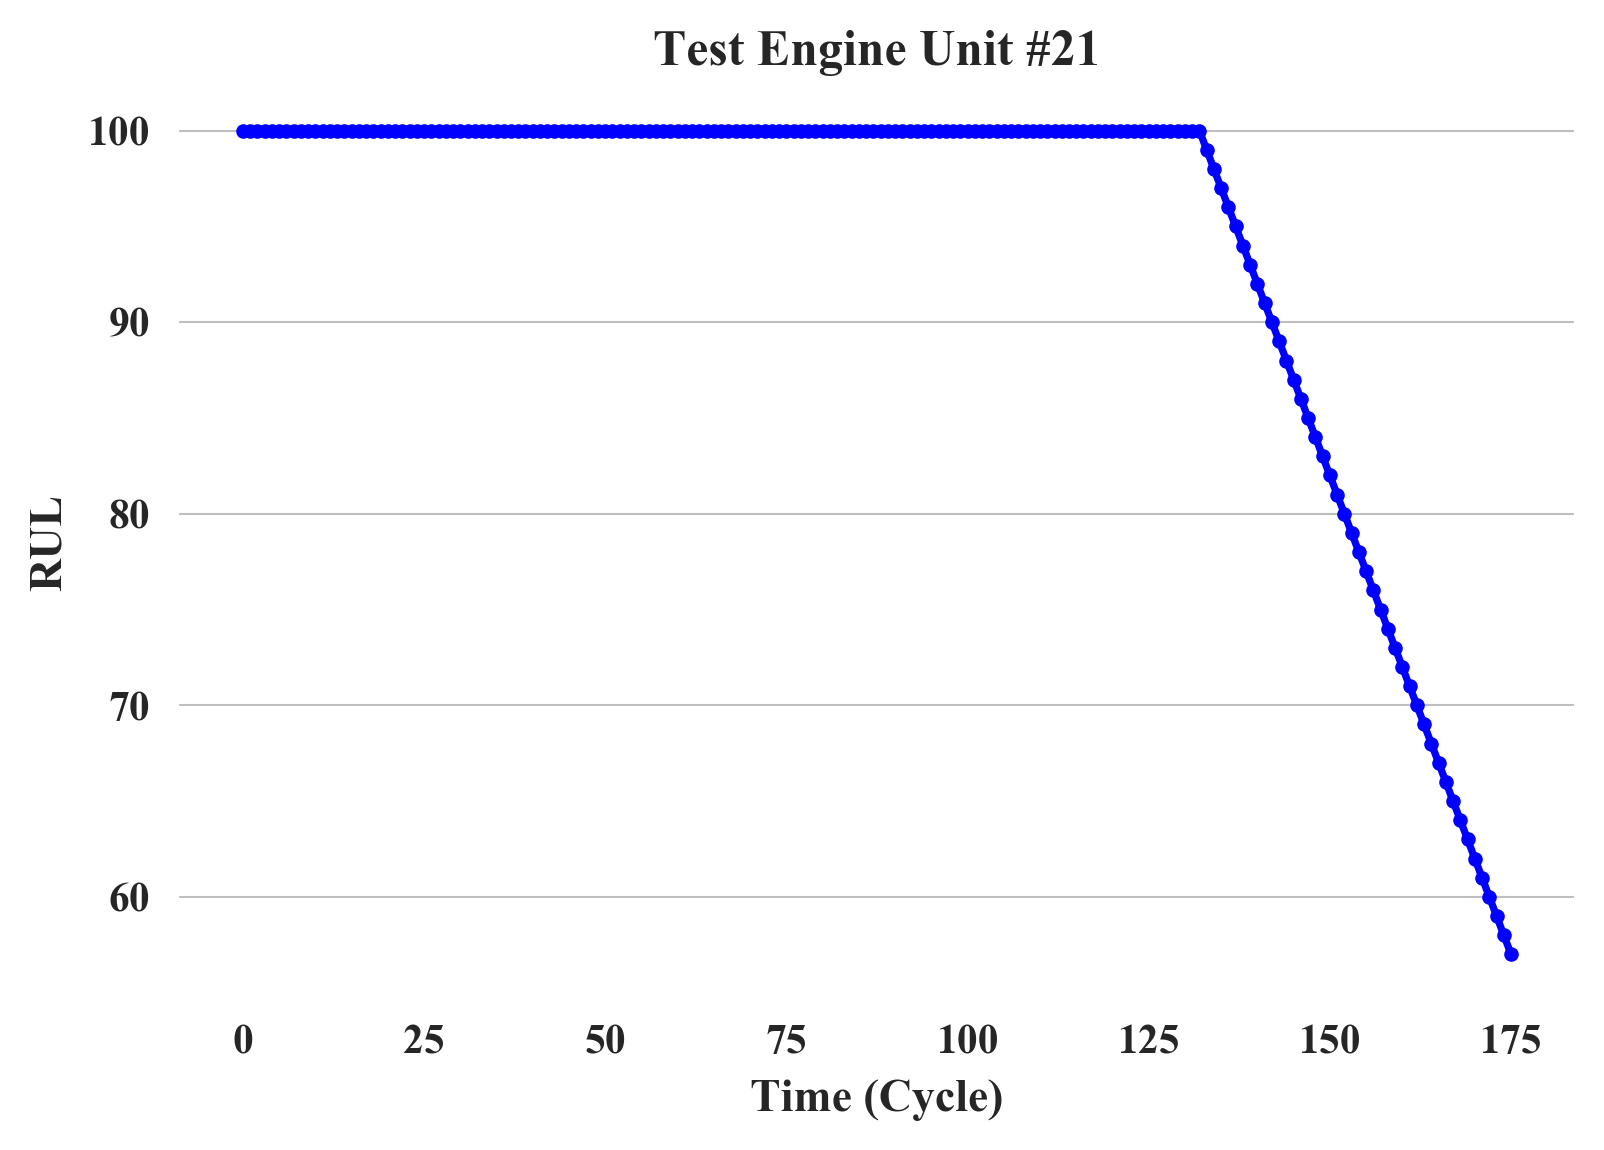
\includegraphics[width=0.7\textwidth]{../img/test_engine.png}
\caption{Piecewise linear degradation for \gls{rul}.}
\label{fig:piecewise_model}
\end{figure}

\subsection{Choosing optimal data-related parameters}
\label{sec:choosing_otimal_data-related_params}

As mentioned in the previous sections the choice of the data-related parameters $v$ has a large impact on the performance of the regressor, i.e. the \gls{mlp}. In this section we present a framework for picking the optimal combination of the data-related parameters $n_w$, $n_s$ and $R_e$ while being computationally efficient.

Recall that $\mathbf{v} = (n_w, n_s, R_e)$, specific to the \gls{cmaps} dataset are the boundaries of each component, i.e. $n_w \in \left[1, b\right]$, $n_s \in \left[1, 10\right]$, and $R_e \in \left[90, 140 \right]$, where all the intervals are integer. The value of $b$ is dependent upon the specific subset, Table \ref{table:b_values} presents the different values $b$ can take for each dataset.

\begin{table}[!htb]
\centering
\begin{tabular}{l | l l l l}
	\hline
	 & FD001 & FD002 & FD003 & FD004\\
  	\hline
  	$b$ & 30 & 20 & 30 & 18\\
  	\hline
\end{tabular}
\caption{Allowed values for $b$ per subset}
\label{table:b_values}
\end{table}

Let also $X(v)$ be the training/cross-val/test sets parametrized by $v$ and used by the \gls{mlp} to perform the \gls{rul} estimation. Finally, let $f(v)=e_{rms}(X(v))$, recall from Equation (\ref{eq:rmse}) that $d = \hat{y} - y$ and that $\hat{y}$ depends on $X(v)$, also note that one function evaluation of $f(v)$ implies training the \gls{mlp} and computing the result of Equation (\ref{eq:rmse}). Here we propose to fine tune $\mathbf{v}$, formally speaking

\begin{equation}
\begin{aligned}
& \underset{v \in \mathbb{Z}^3}{\text{min}}
& & f(v) \\
\end{aligned}
\label{eq:optimization_problem}
\end{equation}

Given the nature of the problem at hand; namely that no analytical form of the problem is given, gradient information is unavailable and the integer nature of the function variables, an evolutionary algorithm is the natural choice for the optimization process.

\subsubsection{Obtaining the true optimal data-related parameters}

The size of \gls{cmaps} dataset and the search space of $v$ allows for an exhaustive search to be performed in order to find the true optimal data-related parameters. We would like to emphasize tough, that although exhaustive search is a possibility for \gls{cmaps} dataset it is in no way a possibility in a more general setting, therefore the use of the evolutionary algorithm (\gls{ea}) adopted in this framework. Nevertheless, the possibility to perform exhaustive search on the \gls{cmaps} dataset can be exploited to demonstrate the accuracy of the chosen \gls{ea} and of the framework overall. Once again, taking subsets $FD001$ and $FD002$ an exhaustive search is performed to find the true optimal values for $v$. As was the case when using \gls{de}, the \gls{mlp} is only trained for $20$ epochs. Table \ref{table:true_optimal_data_params} shows the optimal as well as the worst combinations of data-related parameters and the total number of function evaluations used by the exhaustive search.

\begin{table}[!htb]
\centering
\begin{tabular}{l | c r c r r l}
	\hline
	 Dataset & argmin $v$ & min $f(v)$ & argmax $v$ & max $f(v)$ & Function evals.\\
  	\hline
  	FD001 & $\left[ 24, 1, 127 \right]$ & $15.11$ & $\left[ 25, 10, 94 \right]$ & $85.19$ & 8160\\
  	FD002 & $\left[ 16, 1, 138 \right]$ & $30.93$ & $\left[ 17, 10, 99 \right]$ & $59.78$ & 3060\\
  	\hline
\end{tabular}
\caption{Exhaustive search results for subsets FD001 and F002.}
\label{table:true_optimal_data_params}
\end{table}

\subsubsection{Evolutionary algorithms for obtaining the optimal data-related parameters}
\label{sec:ea_optimization_process}

Evolutionary algorithms (\glspl{ea})/meta-heuristics are a family of methods that optimize a problem by iteratively trying to improve a set of candidate solutions with regard to a given measure of quality. The methods do not make any assumptions about the problem, treating it as a black box that merely provides a measure of quality given a candidate solution. Furthermore \glspl{ea} do not require the gradient of the problem being optimized, making them very suitable for applications such as neural networks. Among the drawbacks of this kind of methods are that they usually require considerable computing effort to converge to a solution.

For this particular application, differential evolution (\gls{de}) \cite{Storn1997} is chosen as the optimization algorithm. Though in principle any meta-heuristic capable of handling integer variables is suitable for this application, \gls{de} has been stablished itself as one of the most reliable, robust and easy to use \glspl{ea}. Furthermore, a ready to use python implementation is available through the scipy package \cite{scipy}. Although \gls{de} does not have special operators for treating integer variables a very simple modification to the algorithm, consisting on rounding every component of a candidate solution $\mathbf{v}'$ to its nearest integer, is used for this work.

As mentioned earlier, evolutionary algorithms such as \gls{de} tend to use several function evaluations for obtaining the optimal solutions, recall that for this application one function evaluations implies retraining the  neural network from scratch. This is not a desirable scenario, as obtaining the optimal data-related parameters $\mathbf{v}$ would entail an extensive use of computational power. Instead of running for \gls{de} for several iterations and with a large population size we propose to run it just for $30$ iterations (generations in the literature of evolutionary computation) and using a population size of $12$, which seems reasonable given the size of the search space of $\mathbf{v}$. 

Furthermore, during the optimization process the \gls{mlp} is not trained for  $100$ epochs, instead the \gls{mlp} is trained for just $20$ epochs, this is done mainly for two reasons: the use of the mini-batch in the training process allows for a speed up in the convergence, therefore it can be assumed that the algorithm will most likely be very close to its optima after just a couple of iterations, second and most important is the assumption that parameters that lead to lower score values in the early stages of the \gls{mlp} training process are more likely to provide better performance when trained for the total epochs. Given the similarities between subsets FD001/FD003 and FD002/FD004 we have decided to just tune the for subsets FD001 and FD002. Details for the use of \gls{de} in finding the optimum data-related parameters are described in Table \ref{table:de_hyperparams}.

\begin{table}[!htb]
\centering
\begin{tabular}{l l l l l}
	\hline
	 Population Size & Generations & Strategy & \gls{mlp} epochs\\
  	\hline
  	12 & 30 & Best1Bin & 20\\
  	\hline
\end{tabular}
\caption{Differential Evolution hyper-parameters.}
\label{table:de_hyperparams}
\end{table}

The optimal data-related parameters for each of the subsets found by \gls{de} are shown in Table \ref{table:optimal_data_params}. As can be observed the results obtained by \gls{de} are in fact very close to the real optima (Table \ref{table:true_optimal_data_params}) in both datasets, nevertheless the computational burden is reduced by one order of magnitude when using \gls{de}. From the results in Table \ref{table:optimal_data_params} it can be observed that the maximum allowable time window is always preferred while, on the contrary, small window strides yield better results, for the case of early RUL it can be observed that larger $R_e$ are favored.

\begin{table}[!htb]
\centering
\begin{tabular}{l | c r r l}
	\hline
	 Dataset & argmin $v$ & min $f(v)$ & Function evals.\\
  	\hline
  	FD001 & $\left[ 24, 1, 129 \right]$ & $15.24$ & 372\\
  	FD002 & $\left[ 17, 1, 139 \right]$ & $30.95$ & 372\\
  	\hline
\end{tabular}
\caption{Data-related parameters for each subset obtained with Differential Evolution.}
\label{table:optimal_data_params}
\end{table}

\subsection{The ANN-EA RUL estimation Framework}

Having described the major building blocks of the proposed method, we now introduce the complete framework in Algorithm \ref{alg:rul_framework}.

\setcounter{algorithm}{0}
\begin{algorithm}[H]
\caption{\gls{ann}-\gls{ea} \gls{rul} estimation Framework}\label{alg:rul_framework}
\textbf{Input:} Initial set of data-related parameters $v \in \mathbb{Z}^n$, Raw training/testing data $X$ and training labels $y$\\
\textbf{Output:} Optimal set of data-related parameters $v^*$
	\begin{algorithmic}[1]
		\State Choose regressor architecture (\gls{ann}, \gls{svm}, linear/logistic regression, etc).
		\State Define $f(v)$ as in Section\ref{sec:choosing_otimal_data-related_params}.
		\State Optimize $f(v)$ using the preferred evolutionary algorithm, i.e. differential evolution, evolutionary strategies, genetic algorithm, etc, using the proposed guidelines from Section \ref{sec:ea_optimization_process}.
		\State Use $v^*$ to train the regressor for as many epochs as needed.
	\end{algorithmic}
\end{algorithm}

%----------------------------------------------------------------------------------------
%	EVAL
%----------------------------------------------------------------------------------------

\section{Evaluating the performance of the proposed method}
\label{sec:rul_eval}

In this section we evaluate the performance of the proposed method. The architecture of the \gls{mlp} to be used here is described in Table \ref{table:proposed_nn} and will be used throughout this section.  The \gls{mlp} was trained $10$ times for $200$ epochs each and tested in each subset of the \gls{cmaps} dataset.

For the first experiment, the combinations of window size $n_w$, window stride $n_s$ and early \gls{rul} $R_e$ are presented in Table \ref{table:data_params_de}.

\begin{table}[!htb]
\centering
\begin{tabular}{l r r r l}
	\hline
	 Dataset & $n_w$ &  $n_s$ & $R_e$\\
  	\hline
  	FD001 & 24 & 1 & 129\\
  	FD002 & 17 & 1 & 139\\
  	FD003 & 24 & 1 & 129\\
  	FD004 & 17 & 1 & 139\\
  	\hline
\end{tabular}
\caption{Data-related parameters for each subset as obtained by \gls{de}.}
\label{table:data_params_de}
\end{table}  

The obtained results for $f(v)$ using the above setting are depicted in Table \ref{table:results_ann_de}. Notice that the performances obtained for datasets FD001 and FD002 improved, this is due to the fact that this time the \gls{mlp} was trained for more epochs, thus obtaining better results.

\begin{table}[!htb]
\centering
\begin{tabular}{l | r r r r | r r r r}
	\hline	
	& \multicolumn{4}{| c}{RMSE} & \multicolumn{4}{| c}{RHS} \\
	Data Subset & min & max & avg & STD & min & max & avg & STD\\
  	\hline
  	FD001 & 14.24 & 14.57 & 14.39 & 0.11 & 3.25 & 3.58 & 3.37 & 0.11\\
  	FD002 & 28.90 & 29.23 & 29.09 & 0.11 & 45.99 & 53.90 & 50.69 & 2.17\\
  	FD003 & 14.74 & 16.18 & 15.42 & 0.50 & 4.36 & 6.85 & 5.33 & 0.95\\
  	FD004 & 33.25 & 35.10 & 34.74 & 0.53 & 58.52 & 78.62 & 74.77 & 5.88\\
  	\hline
\end{tabular}

\caption{Scores for each dataset using the data-related parameters obtained by \gls{de} (Second architecture).}
\label{table:results_ann_de}
\end{table}

\begin{comment}

\begin{table}[!htb]
\centering
\begin{tabular}{l | r r r r | r r r r}
	\hline	
	& \multicolumn{4}{| c}{RMSE} & \multicolumn{4}{| c}{RHS} \\
	Data Subset & min & max & avg & STD & min & max & avg & STD\\
  	\hline
  	FD001 & 13.57 & 15.79 & 14.71 & 0.66 & 3.17 & 4.86 & 4.01 & 0.53\\
  	FD002 & 28.96 & 30.1 & 29.51 & 0.32 & 54.39 & 90.40 & 67.83 & 10.80\\
  	FD003 & 13.88 & 15.89 & 14.68 & 0.81 & 3.14& 5.77 & 4.02 & 0.95\\
  	FD004 & 29.47 & 31.18 & 30.65 & 0.49 & 32.77 & 42.40 & 37.58 & 2.78\\
  	\hline
\end{tabular}
\caption{Scores for each dataset using two sets of data-related parameters (LSTM).}
\label{table:results_lstm_1}
\end{table}

\end{comment}

Next, the possibility of using a single set of data-related parameters for all the subsets is explored. For this experiment the $n_w$ is fixed for all of the four datasets, given that the maximum allowable window size for all datasets is $18$. Hence, the data-related chosen parameters are $v=(17, 1, 139)$, the results obtained are shown in Table \ref{table:results_ann_1}. 

\begin{table}[!htb]
\centering
\begin{tabular}{l | r r r r | r r r r}
	\hline	
	& \multicolumn{4}{| c}{RMSE} & \multicolumn{4}{| c}{RHS} \\
	Data Subset & min & max & avg & STD & min & max & avg & STD\\
  	\hline
  	FD001 & 16.74 & 17.23 & 17.06 & 0.18 & 8.08 & 9.26 & 8.64 & 0.45\\
  	FD002 & 29.77 & 30.12 & 29.94 & 0.11 & 54.90 & 63.53 & 58.82 & 2.39\\
  	FD003 & 16.94 & 18.52 & 17.77 & 0.39 & 6.02 & 10.18 & 7.64 & 1.37\\
  	FD004 & 33.95 & 35.46 & 35.14 & 0.44 & 58.71 & 67.91 & 65.78 & 2.64\\
  	\hline
\end{tabular}
\caption{Scores for each dataset using the single set of data-related parameters.}
\label{table:results_ann_1}
\end{table}

As can be observed, performance is decreased for subsets FD001/FD003, this indicates that larger window sizes are beneficial for this regression problem. Figures \ref{fig:scores_rmse} and \ref{fig:scores_rhs} show a comparison of how the scores are affected for each dataset by changing the data-related parameters to make use of 2 and 1 sets of them.

\begin{figure}[!htb]
\centering
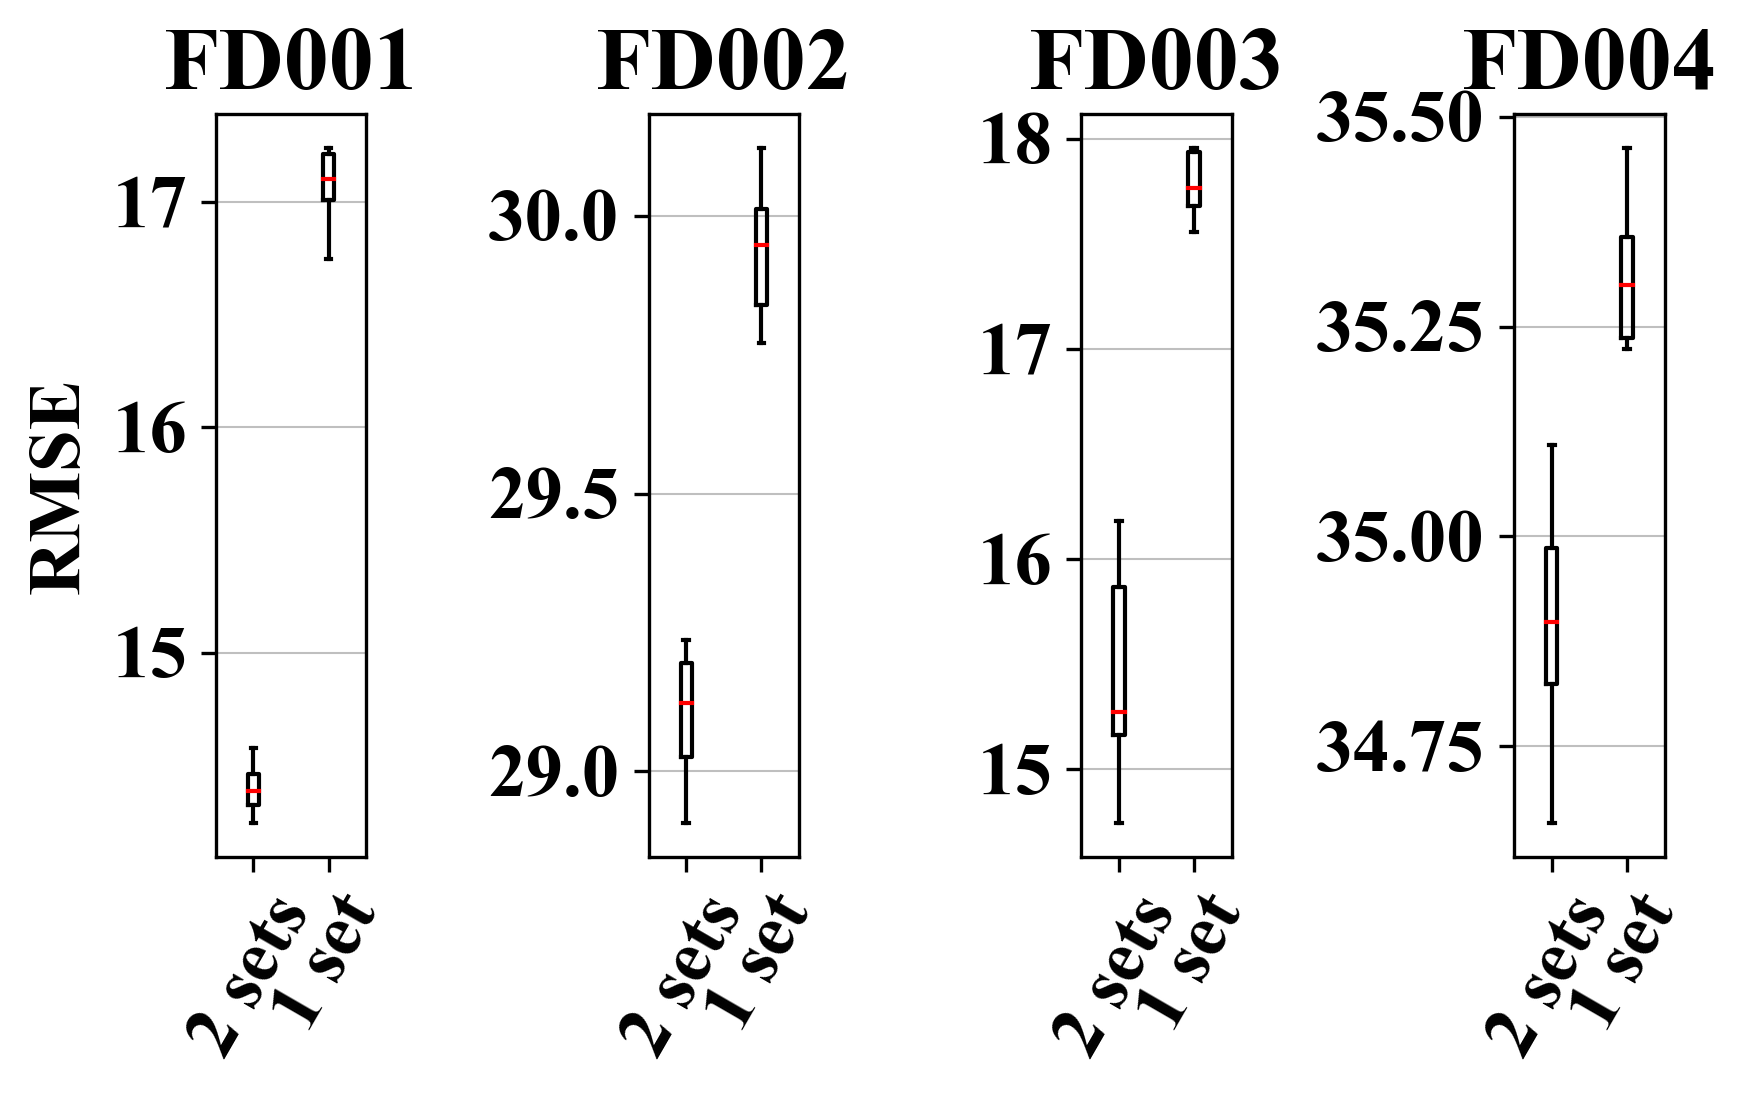
\includegraphics[width=0.7\textwidth]{../img/rmse_comparisson.png}
\caption{Comparison of \gls{rmse} results for different sets of data-related parameters.}
\label{fig:scores_rmse}
\end{figure}

\begin{figure}[!htb]
\centering
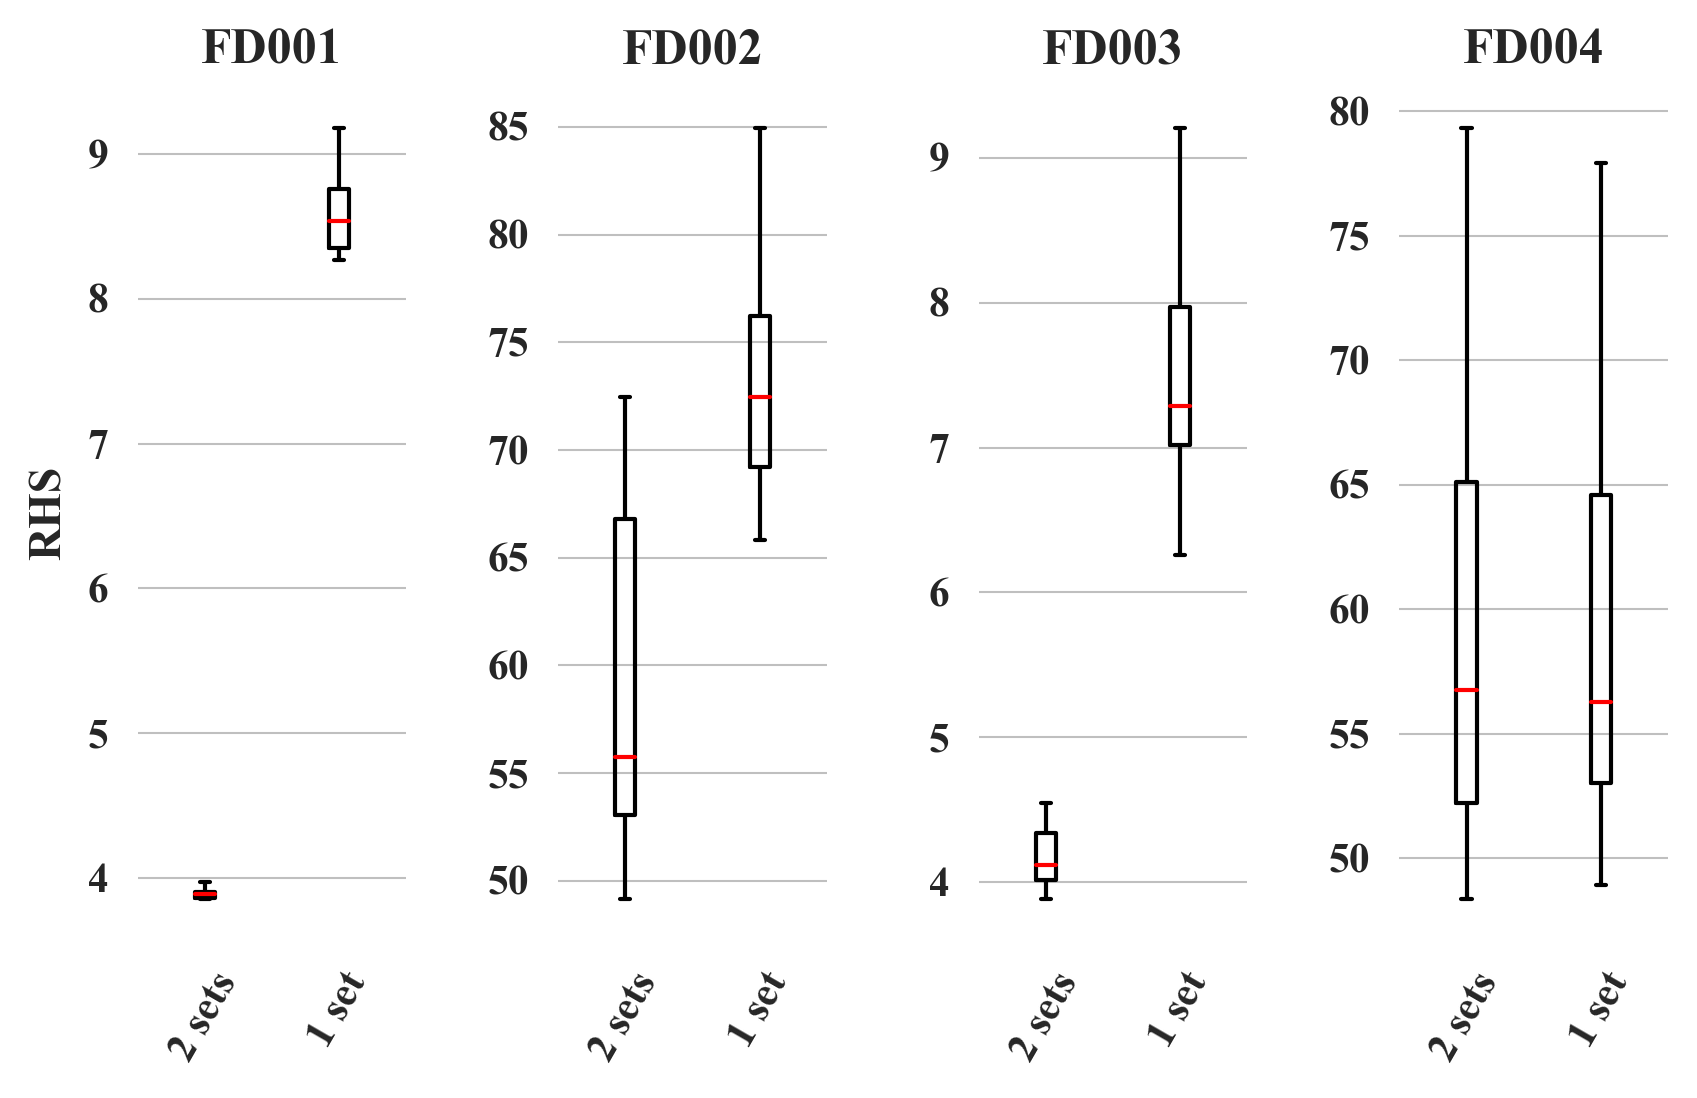
\includegraphics[width=0.7\textwidth]{../img/rhs_comparisson.png}
\caption{Comparison of \gls{rhs} results for different sets of data-related parameters.}
\label{fig:scores_rhs}
\end{figure}

\subsection{Comparison with other approaches}

In this section the performance of the proposed method is compared against other state-of-the-art methods. Most of the presented methods in this section have only reported results on the test set FD001 in terms of $e_{rms}$, the results are displayed in Table \ref{table:results_comparison}. The $e_{rms}$ value of the proposed method in Table \ref{table:results_comparison} is the mean value of 10 independent runs. The remainder of the values are identical to those reported in their respective original papers.

\begin{table}[!htb]
\centering
\begin{tabular}{l | r r r r | r r r r}
	\hline	
	Method & $e_{rms}$ \\
  	\hline
  	ESN trained by Kalman Filter \cite{Peng2012} & 63.45\\
  	Support Vector Machine Classifier \cite{Louen2013} & 29.82\\
  	Time Window Neural Network \cite{Lim2016} & 15.16\\
  	Multi-objective deep belief networks ensemble \cite{Zhang2016} & 15.04\\
  	Deep Convolutional Neural Network \cite{Babu2016} & 18.45\\
  	\textbf{Proposed method with $n_w = 30$, $n_s=1$ and $R_e = 128$} & 14.87\\
  	\hline
\end{tabular}
\caption{Performance comparisons of the proposed method and the latest related papers on the \gls{cmaps} dataset.}
\label{table:results_comparison}
\end{table}

Based on the results, the proposed method performs better than the majority of the compared methods when taking into consideration the whole dataset FD001. Two methods come close to the performance of the presented approach in this paper, namely the time window \gls{ann} \cite{Lim2016} and the Networks Ensemble \cite{Zhang2016}. While the performance of both methods comes close to the results presented in this paper, the presented approach is computationally more efficient. Furthermore, the framework proposed in here is simple to understand and implement, robust, generic and light-weight, features we believe are important to highlight when comparing the proposed method against other state-of-the-art approaches.

%----------------------------------------------------------------------------------------
%	CONCLUSIONS
%----------------------------------------------------------------------------------------

\section{Conclusions and future work}
\label{sec:conclusions}

This paper presents a novel framework for predicting the \gls{rul} of mechanical components. While the method was tested on the jet-engine specific dataset \gls{cmaps}, the method is general enough so that it can theoretically be applied to other kind of similar systems. The framework makes use of a strided moving time window to generate the training and test sets, a shallow \gls{mlp} to make the predictions of the \gls{rul} and an evolutionary algorithm (\gls{de}) which needs to be run just once in order to find the best data-related parameters that optimize the scoring functions used in this study.  The results presented in this paper demonstrate that the proposed framework is accurate and computationally efficient, which makes this framework suitable for applications that have limited computational resources such as embedded systems. Furthermore, a comparison with other state-of-the-art methods shown that the proposed method is the best overall performer. 

Two major features of the proposed framework are its generality and scalability. While for this paper very specific regressors and evolutionary algorithms were chosen, many other combinations are possible and may be more suitable for different applications. Furthermore, the framework here presented can, in principle, be used for model-construction, i.e. generating the best possible neural network architecture tailored to a specific application. Both issues are to be addressed in future work.


%----------------------------------------------------------------------------------------
%	APPENDICES
%----------------------------------------------------------------------------------------
\pagebreak
\appendix
\addcontentsline{toc}{section}{Appendices}
\section*{Appendices}

\section{Tested Neural Network Architectures}
\label{sec:appendices}

Architecture 1

\begin{table}[!htb]
\centering
\begin{tabular}{l l l l}
	\hline
	Layer & Shape & Activation & Additional Information\\
  	\hline
  	Fully connected & 250 & ReLU & L1 = 0.1, L2 = 0.2\\
  	Fully connected & 50 & ReLU & L1 = 0.1, L2 = 0.2\\
  	Fully connected & 1 & Linear & L1 = 0.1, L2 = 0.2\\
  	\hline
\end{tabular}
\caption{Proposed Neural Network architecture 4}
\label{table:proposed_nn_4}
\end{table}

Architecture 2

\begin{table}[!htb]
\centering
\begin{tabular}{l l l l}
	\hline
	Layer & Shape & Activation & Additional Information\\
  	\hline
  	Fully connected & 100 & ReLU & L1 = 0.1, L2 = 0.2\\
  	Fully connected & 50 & ReLU & L1 = 0.1, L2 = 0.2\\
  	Fully connected & 1 & Linear & L1 = 0.1, L2 = 0.2\\
  	\hline
\end{tabular}
\caption{Proposed Neural Network architecture 3}
\label{table:proposed_nn_3}
\end{table}

Architecture 3

\begin{table}[!htb]
\centering
\begin{tabular}{l l l l}
	\hline
	Layer & Shape & Activation & Additional Information\\
  	\hline
  	Fully connected & 50 & ReLU & L1 = 0.1, L2 = 0.2\\
  	Fully connected & 20 & ReLU & L1 = 0.1, L2 = 0.2\\
  	Fully connected & 1 & Linear & L1 = 0.1, L2 = 0.2\\
  	\hline
\end{tabular}
\caption{Proposed Neural Network architecture 2}
\label{table:proposed_nn_2}
\end{table}

Architecture 4

\begin{table}[!htb]
\centering
\begin{tabular}{l l l l}
	\hline
	Layer & Shape & Activation & Additional Information\\
  	\hline
  	Fully connected & 20 & ReLU & L1 = 0.1, L2 = 0.2\\
  	Fully connected & 20 & ReLU & L1 = 0.1, L2 = 0.2\\
  	Fully connected & 1 & Linear & L1 = 0.1, L2 = 0.2\\
  	\hline
\end{tabular}
\caption{Proposed Neural Network architecture 1}
\label{table:proposed_nn_1}
\end{table}

Architecture 5

\begin{table}[!htb]
\centering
\begin{tabular}{l l l l}
	\hline
	Layer & Shape & Activation & Additional Information\\
  	\hline
  	Fully connected & 20 & ReLU & L1 = 0.1, L2 = 0.2\\
  	Fully connected & 1 & Linear & L1 = 0.1, L2 = 0.2\\
  	\hline
\end{tabular}
\caption{Proposed Neural Network architecture 5}
\label{table:proposed_nn_5}
\end{table}

\pagebreak

Architecture 6

\begin{table}[!htb]
\centering
\begin{tabular}{l l l l}
	\hline
	Layer & Shape & Activation & Additional Information\\
  	\hline
  	Fully connected & 10 & ReLU & L1 = 0.1, L2 = 0.2\\
  	Fully connected & 1 & Linear & L1 = 0.1, L2 = 0.2\\
  	\hline
\end{tabular}
\caption{Proposed Neural Network architecture 6}
\label{table:proposed_nn_6}
\end{table}

%------------------------------------------------


%----------------------------------------------------------------------------------------
%	REFERENCE LIST
%----------------------------------------------------------------------------------------

\addcontentsline{toc}{section}{References}
\bibliographystyle{unsrt}
\bibliography{reference_rul_paper}

%----------------------------------------------------------------------------------------

\end{document}
